\newcommand{\OROM}{Id}
\title{What does it take to create with domain-appropriate tools?}
\subtitle{Reflections on implementing the ``Id{}'' system}
\author[ ]{Joel Jakubovic}
\affiliation[ ]{University of Kent, Canterbury}

\maketitle

\newcommand{\joel}[1]{}
\newcommand{\svgel}[1]{\texttt{\textless{}#1\textgreater{}}}
\newcommand{\OSFA}{One-Size-Fits-All}
\newcommand{\xywh}{\texttt{x},\texttt{y},\texttt{width},\texttt{height}}

\begin{abstract}
There is a One-Size-Fits-All{} quality to languages, APIs and even programming itself. Whether you're making a mobile game or a scientific simulation, you will be using a text-based language with similar devices for structuring your code. This is a source of artificial difficulty in creating, understanding, and modifying software systems. No matter the domain, the author's design needs encoding into a form that does not resemble it.

This paper describes a vision where software can be built in a programming environment that is closer to the domain of the software itself. By doing so, users of the system can use familiar abstractions and tools for adapting it. A step towards this vision is presented: a Web version of a minimal OOP system, developed as an executable version of the diagrams of its design, in a substrate meant to facilitate this. The experience of creating such a substrate is analysed, and I suggest deficiencies in programming environments that stand in the way of making this practice commonplace, as well as ways to fill in these gaps.
\end{abstract}

\keywords{substrate, visual, context, domain, adaptation}

\hypertarget{introduction}{%
\section{Introduction}\label{introduction}}

As someone who can code, I have already passed the first and most
important hurdle for making full use of the potential of my computer.
However, even in this supposedly empowered state, I am still far away
from feeling the relationship between myself and software as between
artisan and material, free to shape it into any form with effort
proportional to complexity.

One would have thought that software-creation acts like hypothetical
super-intelligent Artificial Intelligence (AI). That is: even though we
start from a primitive base in the 50s (or even today), there would
surely be a recursive process of self-improvement, building better
software-creation tools with the existing ones, until an ``expressivity
singularity'' where software becomes a workable material as described.

However, this didn't happen. Or at least, it is happening glacially
slowly. The brute fact is that whenever you want to create software, you
go to a text editor and figure out how to translate your design into
that. The text editors, being software, were written with the help of
previous text editors, and so on. It's undeniable that text editors have
improved, even if you think it peaked with Emacs. We just don't seem
able to go beyond them where it matters, such as visual domains
ill-fitted to monospaced ASCII.

Amdahl's Law generalises the following idea: even when you spend hours
of effort doubling the performance of a component used 1\% of the time,
your reward is a system overall improved by a mere 0.5\%. Now, text
coding is certainly ubiquitous, the 99\% case in programming. A small
improvement to text editing, if adopted by everyone, certainly does have
a massive \emph{intermediate} effect---but this only \emph{matters} to
the extent that text was helping us in the first place. If my goal is to
draw or animate pictures, or create a digital synth from a frequency
spectrogram, then giving me the ability to auto-indent my SVG markup is
rather underwhelming as a productivity increase, as it doesn't target
the core of the enterprise that makes it so hard.

As a programmer, I often feel stuck in a box I know I can never escape
from: that box is the text editor, a fixed conduit through which all
\emph{fundamental} changes to my program must pass. It's not a part of
the system I am building, so I can't even make use of features of the
thing I'm developing, to make its own development easier.

Surely the trick is to \emph{use} coding to build something \emph{better
than it}. And then use that, to build something even better. But there
is an enormous breadth and depth of philosophies here, along with all
sorts of concrete systems that failed to catch on. Even worse than this,
is that in my very \emph{language} here I am making the same mistake as
the text editor---speaking in unqualified terms of ``better'' and
``worse'' as if there really is a One-Size-Fits-All{} solution to
software creation!

Of course what we \emph{really} want is the ability for people to create
\emph{in the way that they think is best}\footnote{To be clear: if
  someone \emph{wants} to type out pictures in ASCII, let them---whether
  they do it for a challenge, or even if they find that more natural for
  themselves. But equally, if I want to do it another way, I should have
  that affordance.} in their particular context---to equip them to
feasibly create the tools that suit them for the thing they want to
make. And second-order tools that suit them for making the first-order
tools, and so on. It would do no good to replace text-imperialism with
anything-\emph{else}-imperialism, which is one interpretation of calls
for alternatives.

This dream goes beyond the familiar sense of what constitutes a
``craft'', as far as a strong melding of tool and material. Parallels
can be drawn with industrialisation and a strong division of labour: the
community as a whole produces its higher-order tools, but currently no
single person can have the same autonomy. A (future) software craft
could be expected to give this power to \emph{individuals}, instead of
the community alone. Whenever there are many small specialities
(e.g.~languages, tools, or subject areas) each serving many clients, the
One-Size-Fits-All{} style is the best one can hope for. Adaptation to
individual preferences and idiosyncrasies is only feasible when those
individuals can do it themselves.

What we need is some system that not only lets us create software in a
way that is ``close to the problem domain'' as decided by the
user-developer, but also can augment or change itself to adapt to a
different ``way of creating''. Existing systems seem to only have one of
these properties without the other: Smalltalk and LISP try to minimise
arbitrary commitments of language \emph{semantics} to this end, but
their being textual languages is a fairly tough commitment to break out
of. And it is not so hard to make a specific, \emph{hard-baked} visual
or alternative programming tool---but it is hard to make it
re-programmable \emph{without} having to go back to \emph{its} textual
source code.

All these considerations attract me to the design of a particular system
called ``Id'', as a potential way out of this mess \cite{OROM}. True, it
is a programmer's artefact, but it is still representative of what any
normal person has to do, insofar as:

\begin{enumerate}
\def\labelenumi{\alph{enumi})}
\tightlist
\item
  Wanting to create a piece of software (for whatever reason)
\item
  Having in mind a natural way to represent it as it's being built.
\end{enumerate}

What follows in this paper is an account of how I went about building
Id, atop a preliminary ``box'' substrate.
Section\textasciitilde{}\ref{the-system} gives an overview of Id.
Section\textasciitilde{}\ref{typical-requirements-of-common-software-and-the-work-we-must-do-to-meet-them}
discusses the work involved in obtaining said domain-appropriate
substrate, and Section\textasciitilde{}\ref{patterns-and-polyfilling}
continues with an interpretation of the labour costs of doing this. In
Section\textasciitilde{}\ref{the-system-as-a-part-of-the-solution}, we
return to the Id system and its role in supporting flexible software.
Section\textasciitilde{}\ref{conclusions-and-future-work} addresses the
question in the title, and concludes with next steps for the project.

\hypertarget{the-system}{%
\section{\texorpdfstring{The Id{}
system}{The  system}}\label{the-system}}

When I first read the paper ``Open, Reusable Object Models''
\cite{OROM}, I was hooked on its idea of a small but expressive starting
system that could be self-improved into anything. It describes a
late-bound\footnote{Fewer commitments; more things determined by runtime
  conditions}, Smalltalk-style\footnote{OOP with more emphasis on object
  instances and messaging, as in a distributed system; less emphasis on
  class hierarchies implementing traditional data structures} objects
and messaging environment that the authors call ``Id''.

An Id{} \emph{object} is a block of state which can change as a result
of messages received by it. Messaging (analogous to \emph{method
invocation} in mainstream OOP) works as follows:

\begin{itemize}
\tightlist
\item
  A message is sent by first \emph{bind}-ing its name to its
  \emph{implementation}: specific code, which is then run in the context
  of the receiver \(R\).
\item
  This ``bind'' step is accomplished by sending a further message; this
  time, to the receiver's \emph{vtable} \(V(R)\). A vtable is another
  object that maps ``message name'' to ``implementation code''---it's
  analogous to a ``class'' in mainstream OOP.
\item
  This initial ``bind'' message triggers a similar ``bind'' to
  \emph{its} vtable \(V(V(R))\), and so on: recursing up the
  vtable-chain, and terminating at a base case.
\item
  The higher levels of the vtable-chain mean that different kinds of
  vtables can be supported\footnote{As well as different kinds of
    ``kinds of vtables'', and so on.}, each implementing the ``bind''
  operation in its own way.
\end{itemize}

Inkeeping with its aims of minimality and self-describability, Id as a
whole is ``bootstrapped'' into existence by its initialisation code.
Each step of this code makes use of any parts of the system set up by
the previous steps.

The paper itself consists of mostly prose, several code listings, and
full C sources for a sample implementation at the end. It also provides
several diagrams. But to understand it, I repeatedly found myself
drawing \emph{extra} diagrams.

For example, the first acts of the running system boil down to
initialising the three or so objects. This consists of allocating
memory, interpreting it as a C struct and then filling in fields in a
mundane manner. I had great difficulty following the specifics in my
head, but when I drew tables in the style of their diagrams I readily
saw what what going on. I personally would have preferred these to have
been in the paper in the first place, but I am not necessarily
representative of those who read it\footnote{Besides that, the
  One-Size-Fits-All{} approach is perhaps unavoidable for static print
  media.}.

At any rate, in order to solidify my understanding, there was no better
way than to run the thing and explore it. And yet, having already
``de-compiled'' English text and C source code into object diagrams, it
is a shame to have to compile it all back to struct member assignments.
Worse, the reference system does not even have text I/O when it is run,
let alone some sort of GUI\footnote{That is, the (un)intended user
  interface for Id ends up being a C debugger!}. Faced with the
necessity of adding \emph{some} UI, it seemed a waste of effort to end
up with a system that must be continually polled for its current state
at a terminal prompt.

If I naturally think of this system as 2D tables, why can't that be how
the running system looks? I do not have to keep polling my eyes for what
state my diagrams are in. But further than that---why can't the system
be \emph{built} out of tables in the first place? Shouldn't this be the
main takeaway from the amount of time we spend prototyping, explaining
and designing software as diagrams on paper? Why must the ``natural
representation'' be restricted to the finished product?

Thus was my natural representation decided. My first attempt to make it
a reality was a partial success: a webpage made of HTML tables, evolved
via JavaScript (JS).

\hypertarget{as-html-tables}{%
\subsection{\texorpdfstring{Id{} as HTML
tables}{ as HTML tables}}\label{as-html-tables}}

\begin{figure}[h]
  \centering
  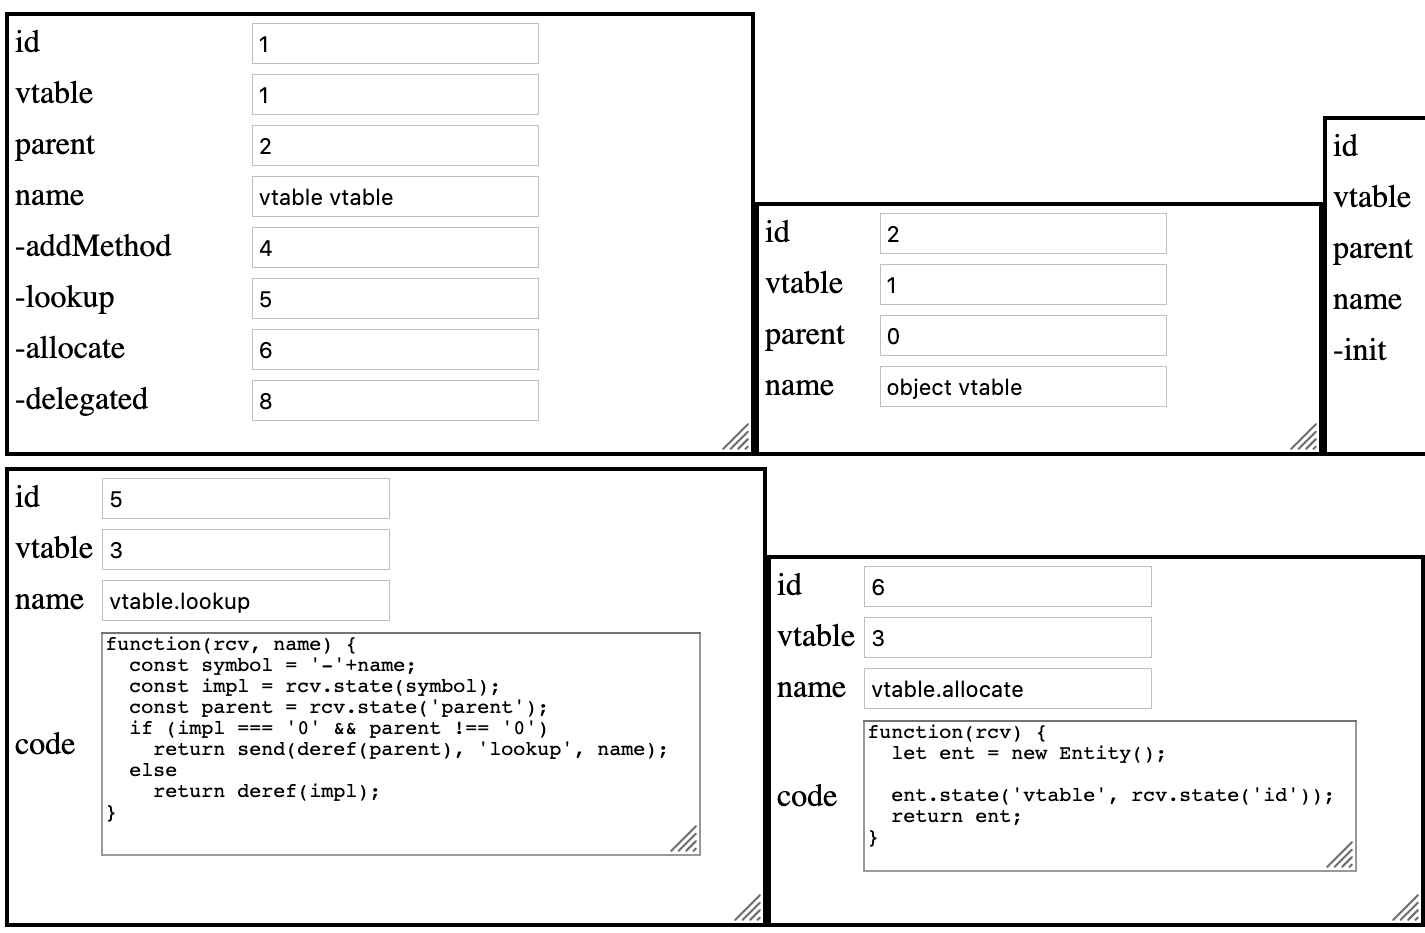
\includegraphics[width=\textwidth]{../orom-html-cropped.png}
  \caption{Part of Id{}/HTML: Obj-dicts are rendered as resizable tables, which reference
           each other through numerical IDs. \label{fig:orom-html}}
\end{figure}

To emphasise the tendency of Id{} objects to be visualised as key-value
mappings, I will refer to them as \emph{obj-dicts}.
Figure\textasciitilde{}\ref{fig:orom-html} shows the Id{}/HTML
implementation \cite{orom-html}, in which they take the form of HTML
tables.

Here, I was grateful for the browser's management of graphical layout,
resizable text fields, and keeping the DOM tree synchronised with what
one sees. This last property enabled me to make the decision to
\emph{directly} encode much of the system state in the DOM, achieving
basic liveness (``The thing on the screen is the actual thing'') for the
keys and values of obj-dicts.

I used a two-column \texttt{\textless{}table\textgreater{}} within a
\texttt{\textless{}div\textgreater{}} for each obj-dict (matching the
diagrams) and gave the rows CSS class names matching the keys (for easy
lookup). Sending messages relied on the JS console, but existing values
in text boxes (such as method implementations) could be edited directly.

This choice of ordinary HTML as a substrate, however, proved rather
two-edged. The browser requires many features to do its job of rendering
complex web pages. And sadly, as its client, I could only make use of
those capabilities which the W3C had decided, at the time of authorship,
were worth the effort exposing in JavaScript. For anything else, the
browser is a black box, and this was very frustrating in the following
case.

\hypertarget{the-radical-concept-of-arrows-that-stay-on-the-shapes}{%
\subsubsection{The Radical Concept of Arrows That Stay On The
Shapes}\label{the-radical-concept-of-arrows-that-stay-on-the-shapes}}

A key aspect of the Id{} system is that there is an object \emph{graph}.
That is, obj-dicts can have entries pointing to other obj-dicts, without
restriction to a tree structure. Drawing arrows to denote this is a
no-brainer (and easy on paper), so I wanted it in my substrate for Id{}.

Luckily, Scalable Vector Graphics (SVG) was at my disposal, which could
be persuaded to display \texttt{\textless{}line\textgreater{}}s over the
\texttt{\textless{}div\textgreater{}}s. But another key feature of my
intended substrate was to be able to rearrange and resize the boxes. So
I would also need to detect changes to the position and size of an
element.

Bizarrely, there is no such facility provided for HTML elements. This,
despite the fact the browser \emph{needs} this functionality hence it
must reside \emph{somewhere} inside the black box.

Reluctantly, I stuck with my plan B: each object has a numerical ID and
pointers are just fields containing a number, followed using a
\texttt{deref()} function.

At this point it was starting to look like a mistake not to have done
the whole thing in SVG. I would gain full graphical freedom, though also
lose some benefits of the browser's managing it on my behalf. I already
knew from experience the surprising complexity of a DIY approach to
layout, model-view updates, and interactivity. But such an exercise
would be an opportunity to carefully observe this tedium, and
crystallise some of my intuitions about why it is so consistently
frustrating.

\hypertarget{as-svg-trees}{%
\subsection{\texorpdfstring{Id{} as SVG
trees}{ as SVG trees}}\label{as-svg-trees}}

\begin{figure}[h]
  \centering
  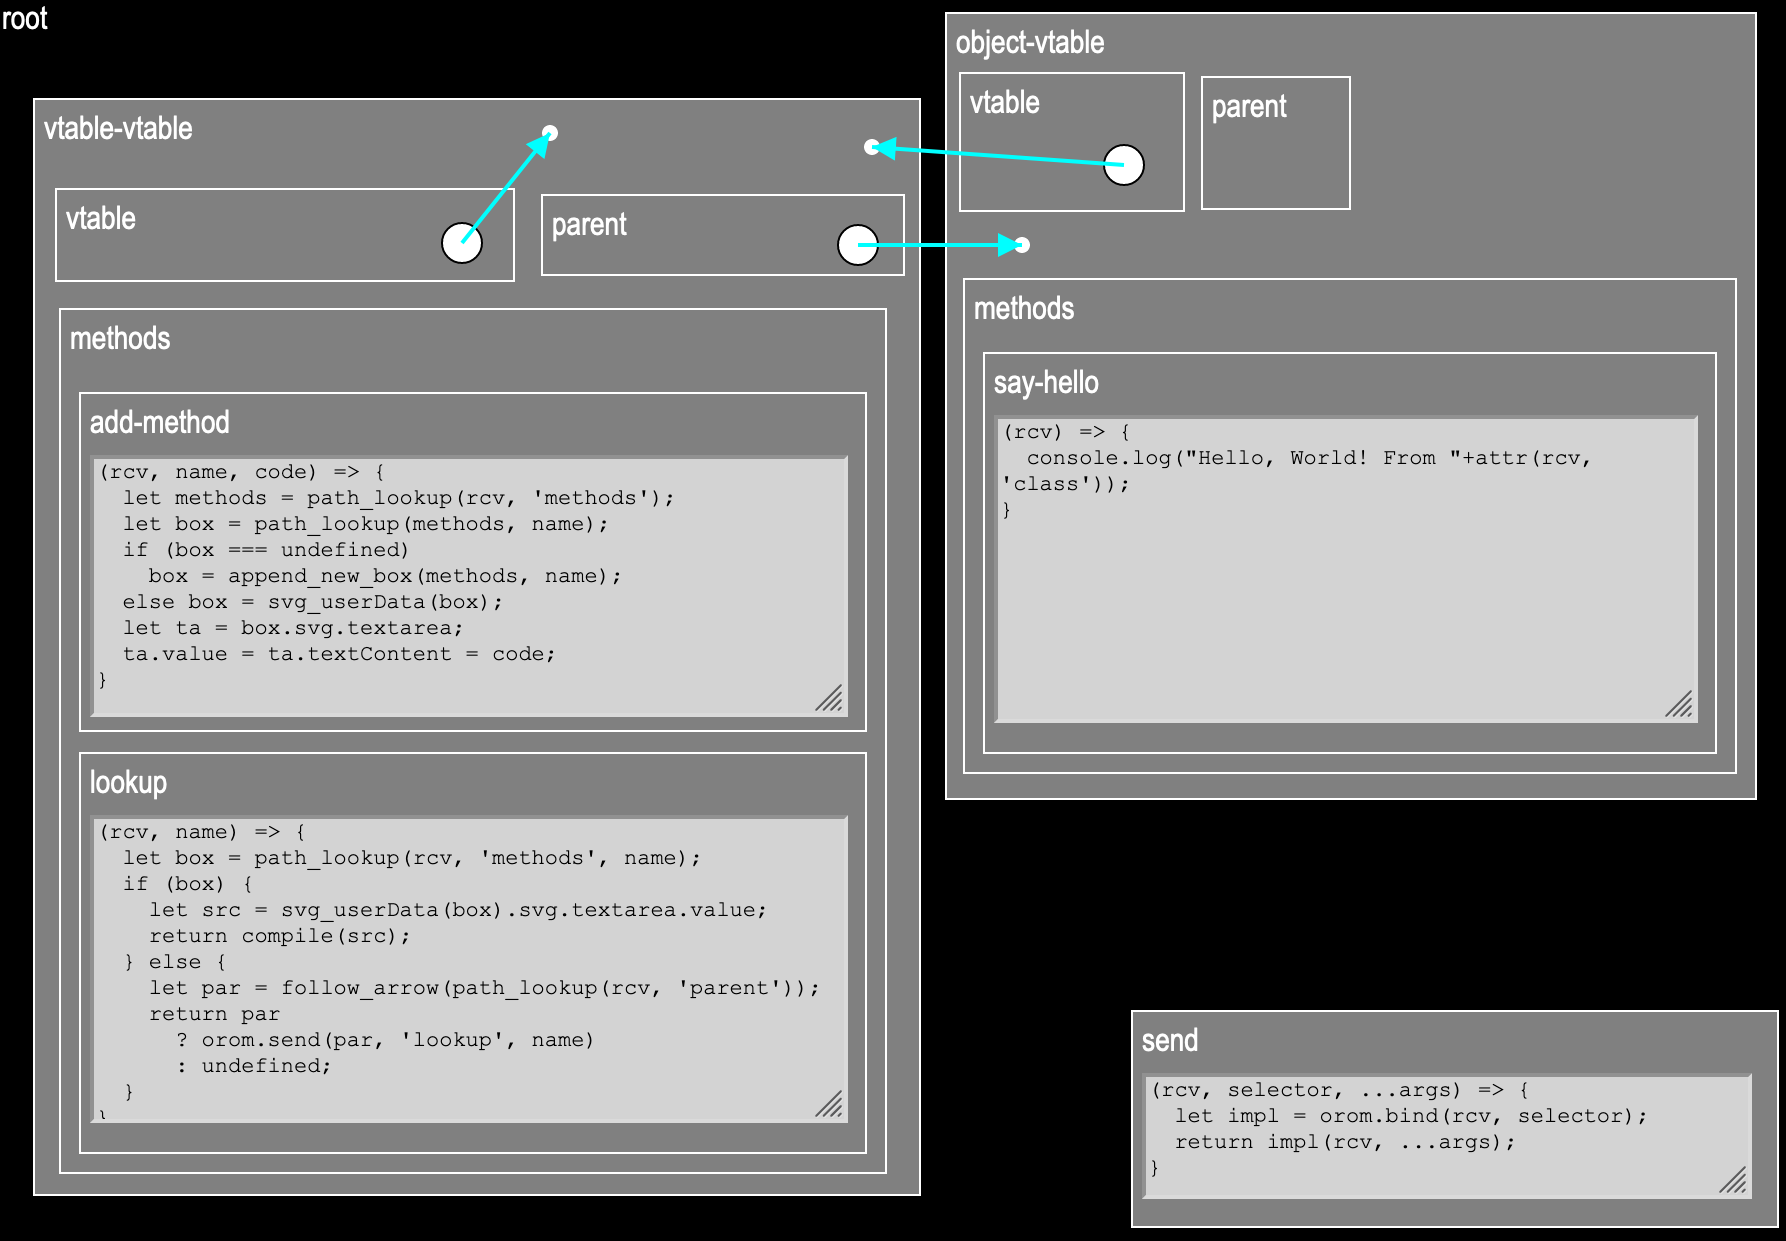
\includegraphics[width=\textwidth]{../orom-svg-cropped.png}
  \caption{Part of Id{}/SVG: Obj-dicts are moveable and resizable nested boxes,
           referencing each other via \emph{real arrows}.\label{fig:orom-svg}}
\end{figure}

In Id{}/SVG, shown in Figure\textasciitilde{}\ref{fig:orom-svg},
obj-dicts are encoded as nested SVG
\texttt{\textless{}rect\textgreater{}}s and other elements, reminiscent
of diSessa's Boxer \cite{boxer}. This was a significant departure from
the table representation, and even though SVG supports (some) nested
HTML via \texttt{\textless{}foreignObject\textgreater{}}, I actually
preferred the possibility of multiple levels of nesting.

Still, this version was far more challenging and took much longer to
reach a satisfactory state. Yet it is precisely this drudgery that
brings me to a better understanding of this paper's question: \emph{what
has it taken?} I shall discuss this in the form of broad patterns or
themes that stand out to me from my development experience, hammered
home by these Id{} implementations.

\hypertarget{typical-requirements-of-common-software-and-the-work-we-must-do-to-meet-them}{%
\section{Typical Requirements Of Common Software (and the work we must
do to meet
them)}\label{typical-requirements-of-common-software-and-the-work-we-must-do-to-meet-them}}

The ``common case'' of software present in our daily lives shares
certain properties, such as being graphical and interactive. Such are
expectations that ``end-users'' hold, consigned as they are to merely
\emph{consume} what programmers give them. But if we want to make
``programming'' more like ``using'', such expectations on \emph{use} at
least need to be acknowledged.

In this section, I will present these and other seemingly
\emph{inevitable} demands of normal software, exemplified by Id{}/SVG. I
will comment on how our programming platforms measure up to the task,
including my chosen platform of JavaScript and Web technologies.

\hypertarget{retained-mode-vector-graphics}{%
\subsection{Retained-Mode Vector
Graphics}\label{retained-mode-vector-graphics}}

Most software is designed for the subset of people who have a colour
display they can perceive. So right away it is going to require ways to
draw coloured shapes. There are usually libraries for this (though they
aren't always \emph{standard} libraries), but some only provide
\emph{immediate mode}: commands to instantaneously rasterise pixels to a
buffer. This is not enough for modern software, as we often expect
animation, or at least to see things change as we interact. Most often
we wish to see \emph{small changes} to the \emph{same} shapes, rather
than completely different shapes altogether; the reification that this
requires to persist between frames, is known as \emph{retained mode.}

On this requirement, SVG fits the bill very well. Although it is not
part of the JavaScript language \emph{per se}, it is a standard and
widely supported technology of the Web \emph{platform}. We can observe
that anyone with a browser \emph{in principle} has access to a powerful
vector graphics editor---just one with no GUI.

The SVG tree has the nice properties of the DOM, such as updating the
display when shape parameters are changed. This is well-adapted to
``I/O-bound'' software like mine, where things change only in response
to user input. If I wanted animation, this would boil down to a regular
``advance simulation'' signal, and would require setting up some
rendering loop. Alternatively, there is the W3C's chosen ontology of CSS
animations, but see
Section\textasciitilde{}\ref{context-appropriate-ontologies}.

\hypertarget{basic-assumptions-about-physical-objects}{%
\subsection{Basic Assumptions About Physical
Objects}\label{basic-assumptions-about-physical-objects}}

In any software making use of vector graphics, there is usually some
level of ``physics'' expected by users. This need not be nearly as
exhaustive as the word ``physics'' might imply, as in e.g.~physics
engines for games; I feel it is important to recognise it for what it is
instead of conceiving physics as an inherently complex thing to be found
only in specialised simulations. For example, pretty much all mobile
apps have what could be called ``phone touch physics'' where menus and
screens slide in and out.

All humans learn a basic set of expectations about the things they see
around them. Some of these, such as ``things fall down'', are not
generally appropriate to software UIs---perhaps because the screen has a
role in our lives a more of a table work surface rather than a vertical
wall, even if it is vertical in real life. The level of physics in
software tends to not involve force, or mass, or very much at all,
merely position and space; we could call it ``geometric physics''.

One thing that all usable software must do, for example, is avoid
crushing many visually complex shapes, such as lines of text, into the
same (unreadable) region. Such concepts of ``solid objects do not
intersect'' or ``only things at different layers may overlap'' are basic
rules inherited from the real world of graphical presentation.

I feel the need to point this out, because by default the computer does
not know even the most obvious things about how space works, so we must
laboriously algorithmise this intuitive concept. This is not only true
in the case of 2-dimensional visual domains, but even in the
1-dimensional case of memory allocation. The physics of 1D memory are
something like this:

\begin{itemize}
\tightlist
\item
  This number range \texttt{0000}--\texttt{FFFF} is like a space
  (addresses = points)
\item
  Every point has at most one owner block (no overlap)
\item
  These blocks are contiguous, finite ranges (1D boxes)
\end{itemize}

Far from being a niche topic in games and graphics, spatial partitioning
algorithms and data structures have surprising relevance to more
ordinary software. Both memory allocation and graphical layout are
essential to today's; shame that only one of those has been recognised
as such---and made part of the standard libraries of programming
languages.

\hypertarget{translationally-rigid-bodies}{%
\subsubsection{Translationally Rigid
Bodies}\label{translationally-rigid-bodies}}

When you have both a screen and a pointing device (e.g.~touch or mouse),
immediately it becomes worth having ways to move things around in at
least a minimally realistic way. We can debate the appropriateness of
Direct Manipulation for various situations. But it does make a lot of
sense in simple cases, such moving around subdivisions of space
(e.g.~windows) or elements of a graphical design.

In Id{}, the obvious candidate for this is the obj-dicts, plus all
nested boxes in Id{}/SVG. If I move the top-level rect, then I expect
its children to move with it. This is simply the translational physics
of \textbf{rigid bodies}: ``this set of points all move together''. Of
course, proper rigid bodies might also rotate and have mass, but this is
usually undesirable for UI elements.

Translational rigidity can be expressed as the points X and Y always
having the same displacement from each other. Or, when one point is
moved, the rest also move by the same delta. This is a problem of
\textbf{preserving the relationship over time}, which was a significant
area of Id{}/SVG.

\hypertarget{maintaining-relationships-over-time}{%
\subsection{Maintaining Relationships Over
Time}\label{maintaining-relationships-over-time}}

The model of state-mutation present in most imperative languages is what
I call ``dumb'' state. The language provides an affordance to change any
part of the state to a new value, but nothing else.

What more could there be? Well, in \emph{every} software system there
are certain rules, or ``invariants'' of \textbf{internal consistency},
such as ``translational rigidity'' above. Often, changes to any part of
the system are permissible, but only if connected or dependent parts of
the state change in response.

The job of keeping track of who depends on whom can fall either on the
programmer, or the computer. If the programmer has to do this, they can
only go so far managing and simulating in their head. As systems grow
more complex, it is only natural to try and make the computer more
intelligent to do this work. What I am building up to is that whenever
we (or I) consider constraints, ``reactive'' programming, or the
``Observer'' pattern as things you only wheel out \emph{on special
occasions}, we only deceive ourselves into doing the \emph{same work}
less explicitly. It seems that such ``live state'' should be the
expected common case for software development.

If a platform does not provide a means to causally link and unlink bits
of live state, then this must form part of the standard boilerplate.
Such was the case in Id{}/SVG: the polyfilled ``Observable'' class is
the most widely used. It wraps a current value and a list of
subscribers, notifying them when it changes.

Getting an object to follow the mouse pointer (e.g.~when dragging) is
\emph{conceptually} very simple: an ``always equal'' relation. In
Id{}/SVG founded on live-state, this can be expressed in much the same
way:

\begin{lstlisting}[language=JavaScript, numbers=none]
subscribe(object.position, pointer.position);
\end{lstlisting}

By default, an Observable A responds to a change from Observable B by
adopting B's new value. So by subscribing the object's position to the
pointer's, pointer movements copy the new position to the object.

\hypertarget{nut-cracking-with-sledgehammers}{%
\subsection{Nut-Cracking With
Sledgehammers}\label{nut-cracking-with-sledgehammers}}

Speaking about vector graphics, physics, layout and constraint
maintenance might give the impression of high \emph{conceptual}
complexity at the heart of even simple software. This is not quite true,
which makes it all the worse that there is yet still immense
\emph{implementation} complexity.

We are conditioned to only think of these in their most general forms.
But the ``vector graphics'' I use in Id{}/SVG are just rects, lines,
circles and text; a fraction of the full capability of SVG. The
``geometric physics'' I use is dwarfed by fully general 2D or 3D physics
engines. The only layout algorithm I had the patience to implement was a
simple way to expand a list of boxes to fit in a new child at the
bottom. The affordance to place and size boxes \emph{manually} is a
convenient substitute, when required infrequently. Yet search for
material on layout algorithms, and it can seem like Fully General Linear
Inequality Solvers like Cassowary \cite{cassowary} are all there is.

The inevitable requirements I suggest here, do \emph{not} necessitate
Fully General anything. In fact, such generality might make it
\emph{more} cumbersome to express what I wanted in Id{}. As the old
wisdom goes, there's no point expressing a simple regex search as an
arbitrary Turing machine; my boxes don't \emph{have} a moment of inertia
or a mass and I don't \emph{need} a linear optimisation solver for my
space management---for the time being. Under the theme of
domain-appropriate tools, I think it is worth designing interfaces for
\emph{smaller-scale} instances of these areas and exploring what they
are still capable of expressing.

\hypertarget{patterns-and-polyfilling}{%
\section{Patterns and Polyfilling}\label{patterns-and-polyfilling}}

The message of the previous section is that existing platforms are often
at the wrong level of abstraction for the requirements of common
software. I recognise that they are reasonably well-adapted to batch
mode file I/O tasks, but that they fail for the \emph{common case} is a
problem. There is largely the same setup per project just to get basic
functionality:

\begin{itemize}
\tightlist
\item
  Here is how I shall describe shapes
\item
  Here is how I make these shapes move together
\item
  Here is how I maintain internal consistency as the user unpredictably
  changes things
\end{itemize}

This burden either falls on the author, or on the wider community to
build and maintain higher-level frameworks, syntax extensions, etc. In
this paper, I refer to this process as ``polyfilling'', with an emphasis
on the DIY, individual level.

It is true, we already have a term for bringing into existence some
software feature that isn't already there: programming. The difference
is that polyfilling is about filling in \emph{boilerplate},
i.e.~functionality \emph{that should have been there in the first place,
but isn't}. This injects some subjectivity and value judgement into the
term. But ultimately, all platforms are designed with certain features
``out of the box'' and leave other features for us to implement ``if
needed''.

When the \emph{normal} problem domain ``requires batteries'', yet the
tools available say ``batteries not included'', it is quite reasonable
to want the batteries to be part of the platform.
Section\textasciitilde{}\ref{what-did-it-take-and-why} will expand on
this further, but here I will list the ``batteries not included'' I
found myself polyfilling in Id{}/SVG.

\hypertarget{wrapping-and-user-data}{%
\subsection{Wrapping and ``user data''}\label{wrapping-and-user-data}}

The classic example of polyfilling is finding that JavaScript arrays do
not support some familiar operation. For example, this used to be the
case with the \texttt{map} function. Yet JavaScript lets you
\emph{directly augment} the \texttt{Array} class with the new operation,
even though \texttt{Array} is ``part of the language'':

\begin{lstlisting}
Array.prototype.map = function() { ... }
\end{lstlisting}

One can do this to all objects, even those of Web APIs. For example, I
use it to connect SVG nodes to the Id{} system: when a
\texttt{\textless{}rect\textgreater{}} is created, it is ``annotated''
with a \texttt{userData} pointer to the box that it is part of. Then,
when clicked, the box can be found immediately.

This could be described as the box ``wrapping'' the
\texttt{\textless{}rect\textgreater{}}, but risks implying that the
\texttt{\textless{}rect\textgreater{}} merely needs to \emph{live
inside}, or \emph{be referenced by}, the box. In this case, the
\emph{reverse} association is also needed (i.e.~mutual pointers); clicks
can only enter the system \emph{through} SVG in the first place. What is
significant here is that JavaScript lets us add such a link to an entity
that \emph{we did not design}.

This term, ``user data'', often crops up in libraries with the same
idea: to associate arbitrary data with an API object. But in languages
that do not permit such \emph{unanticipated} ``annotation'', this has to
be explicitly \emph{designed in} ahead of time. If it wasn't, then it
has to be done in a roundabout way---for example, a separate
\texttt{userData} lookup table, indexed by the memory address of the API
object.

\hypertarget{positioning-and-sizing}{%
\subsection{Positioning and Sizing}\label{positioning-and-sizing}}

The simple desire to move and resize boxes with the mouse motivated a
lot of the concepts in Sections
\ref{basic-assumptions-about-physical-objects} and
\ref{maintaining-relationships-over-time}. This problem could be
considered a microcosm of Id{}/SVG: what's a natural way I
\emph{conceive} of this behaviour, and could I implement it that way?

It starts with a consideration of translational rigidity. In its most
primitive form, this is a relation between two points. Thus it is
natural to draw a line or ``rod'' between them. It seems that this rod
transmits changes in one of its endpoints directly to the other
endpoint. Since they both feel the same deltas, the displacement vector
between them is preserved
(Figure\textasciitilde{}\ref{fig:delta-transmission}).

\begin{figure}[h]
  \centering
  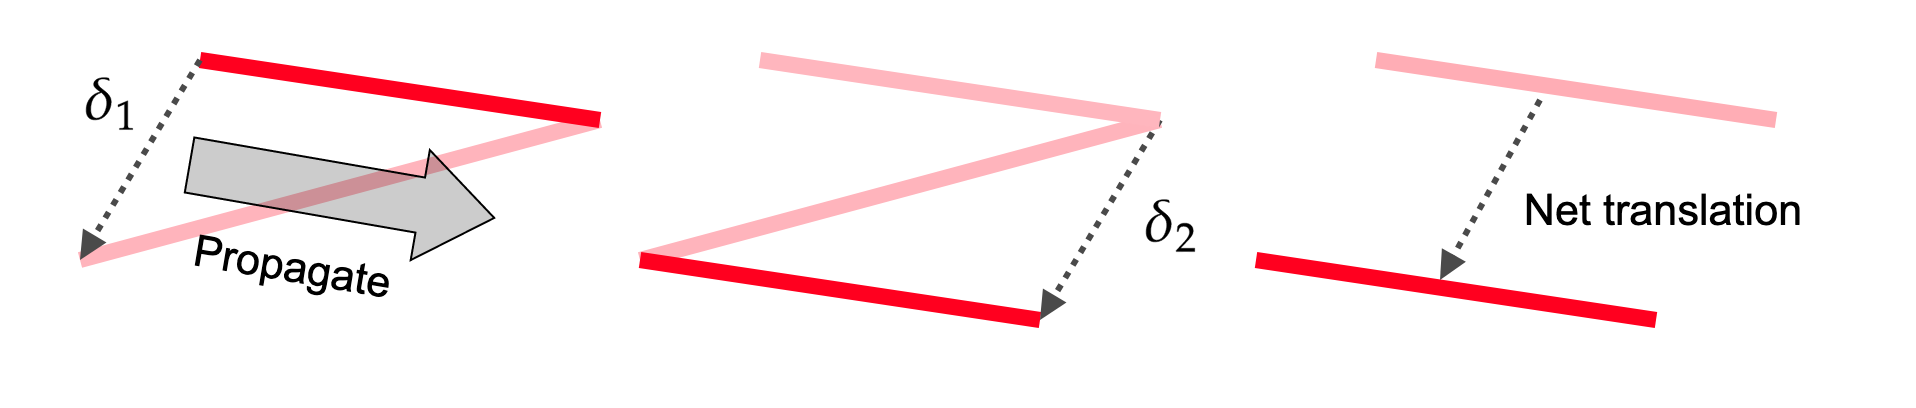
\includegraphics[width=\textwidth]{../delta-transmission.png}
  \caption{Fully rigid rods transmit changes in one end to the other end. \label{fig:delta-transmission}}
\end{figure}

I like to see what I'm doing, so I wanted these rods to be visible and
thus somehow \emph{present in the SVG}. For this, I have a Point class
that is used wherever manipulable points (SVG circles) are needed, and a
Rod class that draws a \texttt{\textless{}line\textgreater{}} and
transmits endpoint deltas across its length.

Resizing of boxes could be achieved through rods that stay horizontal or
vertical. In the language of ``small differences'' spoken by the
live-state infrastructure, this is expressed as a rod ``transmitting
deltas'' in the vertical and horizontal, ``absorbing'' the other
component into itself (Figure\textasciitilde{}\ref{fig:rods}). Mirroring
a DOM rect to these rods is as simple as subscribing its width and
height to horizontal and vertical rods' \texttt{length} Observables.
This way, boxes can be resized from whatever corner is convenient.

\begin{figure}[h]
  \centering
  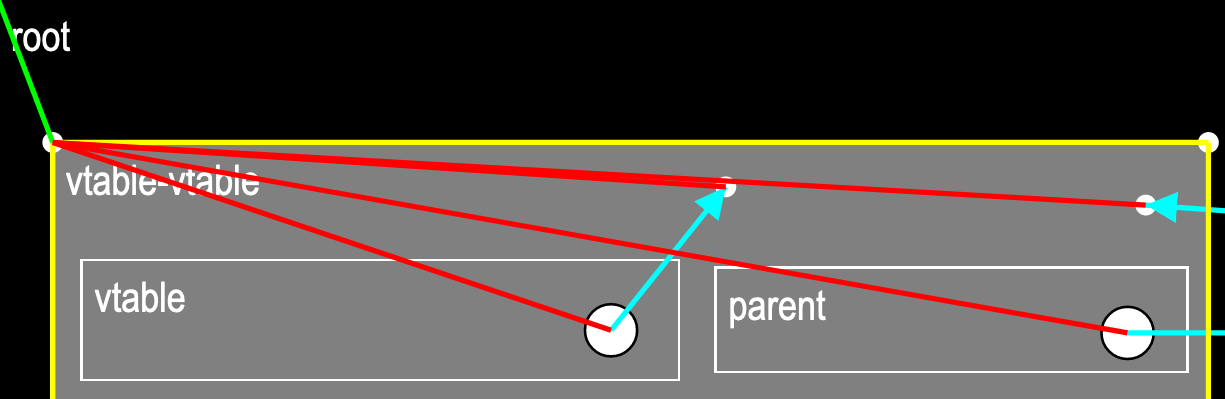
\includegraphics[width=\textwidth]{../rods.png}
  \caption{The yellow rods on the box border are ``half-rigid'': they transmit horizontal or vertical changes, but not both. The green rod in the top-left absorbs all changes from an endpoint into itself, visualising the displacement vector of the child box from its parent. The remaining red rods are fully rigid. A line of CSS can reveal this ``scaffolding'' which is normally hidden for users. \label{fig:rods}}
\end{figure}

Unfortunately, with these rods came possibly the most frustrating
technical challenges of the entire system. Initially I hoped to move
boxes as rigid bodies by temporarily making their border rods rigid.
However, the four border rods form a cyclic graph, as rods are not
directed. This, coupled with the unintended depth-first semantics of
Observable notification (a result of JavaScript function calls in a
loop), led to duplicate deltas applied twice and other nightmares. This
is the tip of an entire research iceberg stretching from Functional
Reactive Programming to internet routing and distributed algorithms.

I had to shelve this investigation in the interest of continuing with
the rest of the system, but I did manage to surmount this through
kludging and compromise. So I do not know whether these problems are
merely a consequence of some design decision I could change to escape
it, or if they are intrinsic to my (modest) UI goal.

\hypertarget{visible-coordinate-systems}{%
\subsection{Visible Coordinate
Systems}\label{visible-coordinate-systems}}

Rigidity in a flat world of sibling shapes is somewhat straightforward.
However, rigidity in the SVG world is more involved.

First of all, SVG shapes (e.g.~\texttt{\textless{}rect\textgreater{}})
are strictly \emph{leaf} nodes of the DOM. So if I wish to nest boxes
within boxes, the visible box \texttt{\textless{}rect\textgreater{}}
must be a mere \emph{accessory} to the nestable element, in my case a
\texttt{\textless{}g\textgreater{}} (group). This means that instead of
resizing the \texttt{x}, \texttt{y}, \texttt{width}, \texttt{height}
attributes of the \texttt{\textless{}rect\textgreater{}}, only its
\texttt{width} and \texttt{height} change, along with the
\texttt{transform} attribute of its \emph{parent}
\texttt{\textless{}g\textgreater{}}. This was not too bad; just
subscribe this attribute, instead of the
\texttt{\textless{}rect\textgreater{}} position, to the top-left Point
handle.

All child elements of a node transform with it, so already SVG has baked
in a basic facility for translational rigidity. This is only available
as a tree hierarchy\footnote{This highlights the mismatch between the
  tree-based DOM and any system that is graph-structured.}, but it is
still useful. However, it conflicts with my early decision to have Point
objects all share the global co-ordinate system (this was to ensure that
simple relations, such as a point following the mouse pointer, are not
infuriating to express.) Still, it was necessary in the case of certain
elements---especially those which must transcend the tree structure
altogether, like arrows between boxes---to bite this bullet, one way or
another.

Again, I return to how we tend to work things out in the freedom of
paper. Co-ordinate systems, here merely positionally displaced, have
their origins here and there and have vectors between them. The rods
thus far let me visually express relations between global Points; now
was a question of expressing one global Point as a displacement from
another (the \texttt{\textless{}g\textgreater{}} transform). New rod
Observables \texttt{p2\_from\_p1} and \texttt{p1\_from\_p2} do the
vector subtraction, which can then be propagated as local co-ordinates
to children. It is nice to express the relation (as well as see it!)
this way (Figure\textasciitilde{}\ref{fig:rods}).

\hypertarget{context-appropriate-ontologies}{%
\subsection{Context-appropriate
ontologies}\label{context-appropriate-ontologies}}

Each API has its own conventions, including a way of naming and
structuring expressions: an \emph{ontology} \cite{crit-semprola}. The
One-Size-Fits-All{} approach is exemplified in such interfaces.

In SVG, we express a rectangle by
\texttt{\textless{}rect x="10" y="10" width="600" height="400"\textgreater{}}.
The SVG specification \emph{defines} to the user that a rect simply
\textbf{is} a top-left corner, a width, and a height---and that's it.
However, this SVG-approved parametrisation of a rectangle is far from
the only one, and thus is, unsurprisingly, ill-fitted to some contexts.

I find it natural to resize boxes by dragging any of their four corners,
so I wanted this in Id{}/SVG. In this context, a ``rectangle'' is
\emph{seen as} four points: top-left, top-right, bottom-left,
bottom-right. Obviously this is not a \emph{minimal} description, since
given e.g.~the top-left and bottom-right, the other two points can be
inferred. But one way or another, to be able to drag any of them, all
four points must be present at \emph{some} level. This alternative
ontology was polyfilled in the form of a ``rect controls'' class that
can be attached manually to any SVG
\texttt{\textless{}rect\textgreater{}}. The \texttt{x} and \texttt{y}
are subscribed to the top-left Point\footnote{In the usual case where
  the \texttt{\textless{}rect\textgreater{}} is part of a box, the
  top-left instead controls the parent
  \texttt{\textless{}g\textgreater{}}'s \texttt{transform}---but the
  idea is the same.}; \texttt{width} and \texttt{height} are subscribed
to Rod lengths.

Another example is to be found in the DOM's event listener model.
Conceptually, many ``events'' are in fact changes to the state of some
physical device. And both keyboard keys and mouse buttons, for example,
have two states---pressed, not pressed---which ought to make them
\emph{interchangeable} to some extent. Indeed, this is why there is such
a thing as ``key mapping''\footnote{For example, the player can
  re-assign the action ``shoot'' from its default mouse button to a
  keyboard key, or another action from keyboard to mouse, as it suits
  them.} in PC games. But the official ontology of the Web makes it
nontrivial to do this.

To start with, the situation is modelled not as the \emph{changing} of
some time-varying property, but instead as a sort of Cartesian product
of subroutines. Rather than, say, a piece of live-state for the left
mouse button (LMB), we get \texttt{onmousedown} and \texttt{onmouseup}.
Thankfully we do not have \texttt{onAdown}/\texttt{onAup},
\texttt{onBdown/onBup}, \ldots{} all the way to
\texttt{onZdown}/\texttt{onZup}, but only
\texttt{onkeydown}/\texttt{onkeyup}. Yet this is just one of the many
possible ways to slice this 3-dimensional\footnote{Device (mouse,
  keyboard), sub-device (button, key), state (up, down)} space.

In Id{}/SVG I did not quite want to re-map keys, but I did often want to
have things follow the mouse when dragged. In order to do this, I
reified the mouse pointer and its position, letting me write
\texttt{subscribe(point.position,\ pointer.position)}. The Point has an
\texttt{is-considering-me?} Observable wrapping
\texttt{onmouseover}/\texttt{onmouseout}, and the LMB is reified into
\texttt{left\_mouse\_button\_is\_down} to be explicit. The
aforementioned subscription is set up whenever
\texttt{is-considering-me?} and \texttt{left\_mouse\_button\_is\_down}
become true, and torn down otherwise. I tended to think of this in the
form ``subscribe to pointer \emph{only when} pointer is-considering-me
\emph{and} LMB is down'', but I could live with this notation as a
future polyfill in JavaScript.

The way these things are connected to the browser's event listeners
could be called ``device drivers''---an approach described in
\cite{prog21-bbox}. It amounts to translating information from the Web's
ontology into that of my substrate, as early as possible:

\begin{lstlisting}
svg.onmousedown = e =>
  if (e.button === 0) change(left_mouse_button_is_down, true);

svg.onmouseup = e =>
  if (e.button === 0) change(left_mouse_button_is_down, false);

svg.onmousemove = e => {
  let r = svg.getBoundingClientRect();
  let pos = vsub([e.clientX, e.clientY], [r.left, r.top]);
  change(pointer.position, pos);
};
\end{lstlisting}

It takes some frustration and experience to get used to the idea that
you have a right to polyfill in alternative representations. Before I
came to this conclusion, I used to twist my head around translating my
intention into the
\texttt{x},\texttt{y},\texttt{width},\texttt{height}{} parameters, and
un-translating when reading back the code I had produced. Once you get
used to having to adapt your mental imagery to a single way of doing
things (i.e.~learning to code), it makes sense to simply expect to see
more of it---especially when you know you are new, surrounded by
veterans who see no problem, and so on. Nowadays, I take the position
that these are simply \emph{widespread} failings of our way of doing
things, instead of \emph{our} failure to adapt to the way software is.

What would it look like to support multiple ontologies? Naïvely, there
are two answers: anticipate the possibilities ahead of time, or support
users adding their own. It is unclear if we can do better on the latter
than simply ``support polyfilling''. As for the former, anticipating the
diversity of ways someone might look at the world is generally doomed to
fail. But in the special case of fairly \emph{formalised} concepts such
as geometrical shapes or mathematics, I could suggest that simple
\emph{under-specification} is the root of the problem in SVG. Instead of
the specification explaining in English that ``\texttt{x} and \texttt{y}
are the co-ordinates of the top left-hand corner\ldots{}'', it might be
better to make these relations machine-readable or \emph{embodied} in
the API. For the rect this might look like:

\begin{itemize}
\tightlist
\item
  A \texttt{rect} is\ldots{}
\item
  a \texttt{polygon} (to be defined elsewhere)
\item
  defined by 4 \emph{degrees of freedom} \texttt{x\ y\ width\ height}
  (internal representation)
\item
  where there are 4 \emph{vertices}, all \texttt{point}s

  \begin{itemize}
  \tightlist
  \item
    \texttt{{[}x,y{]}} called \texttt{top-left}
  \item
    \texttt{{[}x+width,y{]}} called \texttt{top-right}
  \item
    \texttt{{[}x,y+height{]}} called \texttt{bot-left}
  \item
    \texttt{{[}x+width,y+height{]}} called \texttt{bot-right}
  \end{itemize}
\end{itemize}

The hope is that if we then specify enough information---say, the
bot-left and top-right---then the runtime has all it needs to derive its
internal 4 degrees of freedom.

In a crude sense, I have successfully anticipated the most obvious
ontologies of a rectangle here. However, I missed out the ``centre plus
half-width and half-height'' formulation, among others. Is this a futile
effort even for precise mathematical knowledge structures, or could
enough formalisation\footnote{A related question is whether type systems
  and other auto-reasoning formalisms are trapped in a doomed quest for
  ``closed-form'' AI, representable as a \LaTeX~formula.} of Euclidean
geometry in the Web platform put an end to this sort of polyfilling?

There is, in fact, a part of the SVG specification \cite{svg-rect} that
comes \emph{frustratingly close} to the above. It spells out how the
\texttt{\textless{}rect\textgreater{}} parameters ``reduce'' to more
primitive line-drawing steps, including expressions for the four corners
in terms of \texttt{x},\texttt{y},\texttt{width},\texttt{height}{}. The
problem is, this reduction is still described in \emph{natural language}
for a human implementor, missing the potential of such a
formulation\footnote{The point here is that a machine-readable
  description could easily remain human-readable, but a natural-language
  description is not easily machine-readable.}.

It is worth admitting that there is is a significant shortcoming of my
polyfill here, and perhaps throughout. It has taken the form of
\emph{overriding} the default ontology, \emph{replacing} it with the one
I preferred. From my perspective, this is fine. But if another person
were to join in the development of Id{}/SVG, they would be stuck in the
same situation I was in, unless they fully agreed with my ontologies.

The desideratum of ``ontology co-existence'' is very much an open
research problem. \cite{crit-semprola} gives a taste of the thorny
complications unaddressed by a ``Semiotic Programming'' solution
\cite{semprola}, while \cite{kell-c} points out how the idea of
``linking'' is unconcerned with whatever language compiled to the object
code; language-agnosticism is one salient example of ontology
co-existence. This is especially clear if we agree with the latter
author's view that ``which language'' ought to be an
\emph{implementation detail}, that languages ought to be treatable as
\emph{different views} onto the same thing.

These considerations did not occur to me because this project is very
idiosyncratic to my interests, at least in its initial stage. I always
worked on the assumption that I was the only developer. However, a
future Id{} system in a mature state should by no means be bound to this
fact. It is also worth considering \emph{myself in the future} as a
different agent, with different ontology preferences. In that case, the
method here will need to be re-examined.

\hypertarget{extensional-functions}{%
\subsection{Extensional Functions}\label{extensional-functions}}

Time and time again we come across the same pattern of partitioning
system state: trees or graphs of dictonaries, a.k.a. Maps, a.k.a.
associative arrays. I am talking about filesystem paths
\texttt{/path/to/some/file}, Python / Java modules
\texttt{com.example.pkg.subpkg}, JavaScript objects
\texttt{window.my\_obj.component}. The common case is an association of
a textual name to an arbitrary value. I find it useful to see this as a
mathematical ``function'' defined \emph{extensionally} by listing its
input/output mappings---this opposed to an \emph{intensional} definition
such as \(x \mapsto 2x+3\), or a computer program.

Extensional functions are perhaps the most basic form of Knowledge
Representation, and match natural language very well. ``The bicycle's
wheels' spokes are silver'' straightforwardly translates to a function
equation

\begin{lstlisting}
root (bicycle) (wheels) (spokes) (colour) = root (silver)
\end{lstlisting}

That is, whatever object is the output of \texttt{silver} in the
top-level \texttt{root} function, the output of \texttt{colour} (in the
function on the left) points to the same object. The ability to
partition a system in this way enables what \cite{externalise} calls a
``natural co-ordinate system'' for a piece of software, crucial for
understanding and adaptability by others.

It seems that this way of expressing the ``parts'' of a system is an
inevitable requirement of any programming substrate. Some languages,
such as C, do have static, \emph{compile-time} associative arrays
(\texttt{struct}s). In my experience this is usually not enough, and
it's necessary to bring in a library or clutter the code with a
home-grown approximation to dynamic ones. Some parts of the Id{}
authors' C code were confusing until I realised they were just the guts
of a basic associative-array implementation; when I switched to
JavaScript, these lines vanished.

Perhaps another strength of JavaScript is its low \emph{concrete syntax
cost} for \emph{instances} or \emph{literals} of associative arrays.
Writing or reading

\begin{lstlisting}
a = {
  b1: { c1: z, c2: y },
  b2: { c3: x, c4: w }
};
\end{lstlisting}

is more ``What You See Is What You Get'' than the imperative-style

\begin{lstlisting}
a = new Map();
a.set('b1', new Map());
a.get('b1').set('c1', z);
a.get('b1').set('c2', y);
a.set('b2', new Map());
a.get('b2').set('c3', x);
a.get('b2').set('c4', w);
\end{lstlisting}

The latter style is unfortunately still required in JavaScript for
extensional functions with \emph{non-string} inputs.

My original flat, tabular representation in Id{}/HTML did support a
single level of such ``extensional functions'', but no more. In other
words, the output of such a mapping could not be a further mapping
itself. This was problematic because vtables, conceptually, have two
levels of such nesting: the top-level fields, and the ``methods
dictionary'' which contains its own input-output pairs. To distinguish
between these, I actually stored method mappings with an ad-hoc ``-''
character (Figure\textasciitilde{}\ref{fig:method-hyphens}).

By contrast, after switching to the fully nestable box substrate in
Id{}/SVG, I could directly express the model I was thinking in. Quite
simply, the \texttt{vtable} box has a \texttt{methods} box, and that's
where the method boxes go (Figure\textasciitilde{}\ref{fig:orom-svg}).
If I had stayed in HTML, there is a good risk I would have had to
polyfill in extensional functions---whether through nested
\texttt{\textless{}table\textgreater{}} elements, additional ``-''
characters, or something else.

\begin{figure}[h]
  \centering
  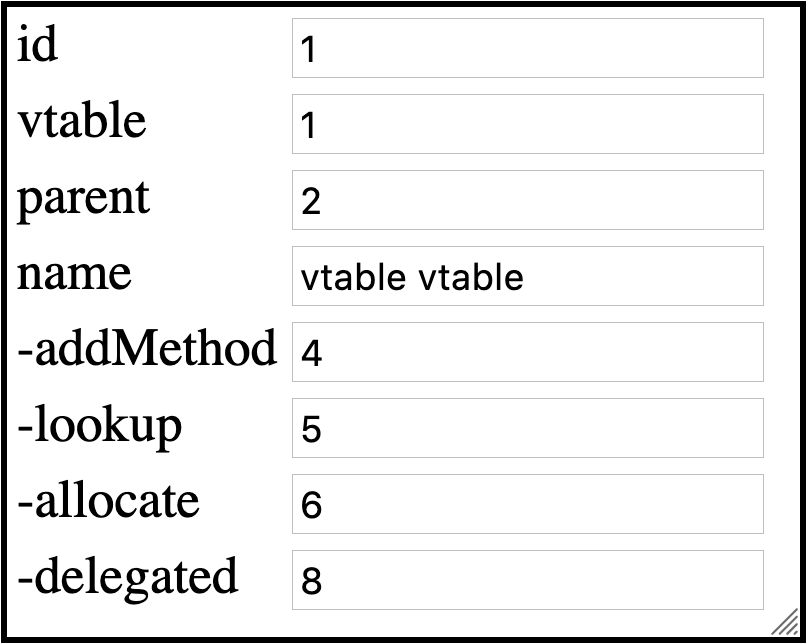
\includegraphics[width=0.5\textwidth]{../method-hyphens.png}
  \caption{Id{}/HTML: use of hyphenated \texttt{-lookup} to signify a \emph{method} called
           \texttt{lookup} instead of a property like \texttt{vtable}. \label{fig:method-hyphens}}
\end{figure}

\hypertarget{persistence}{%
\subsection{Persistence}\label{persistence}}

This refers to exposing structured program state to the user. This data
can then be saved and used to restore the system at a later date, but it
can also be tweaked with corresponding changes reflected in the system.

Persistence was absolutely necessary to continue Id{}/SVG development,
past a certain point. This is because, upon discovering a bug and fixing
it in the source code, the web page must be refreshed and started anew.
In the beginning, when verifying that box drawing with the mouse is
working correctly, this is not much of a problem: upon refresh, the
blank initial state is restored and I could draw again. But as the
substrate matured, and I began to implement parts of the target system
(Id{})---the cycle of finding a bug, tearing down the system, refreshing
and losing work, and manually building it up again, proved frustrating.
Because the system could only be patched externally and restarted, there
needed to be some way to persist changes which live in the DOM, rather
than the source files.

Normally, this can be as simple as autosave to the filesystem. But the
Web platform is very wary of this\footnote{As anyone who learns WebGL
  can attest to, when they discover they must run a local Web server to
  provide image files for textures since any filesystem requests will be
  rejected for security.}, so the solution I turned to was manually
copying the markup in the browser's inspector
(Figure\textasciitilde{}\ref{fig:html-inspector}).

\begin{figure}[h]
  \centering
  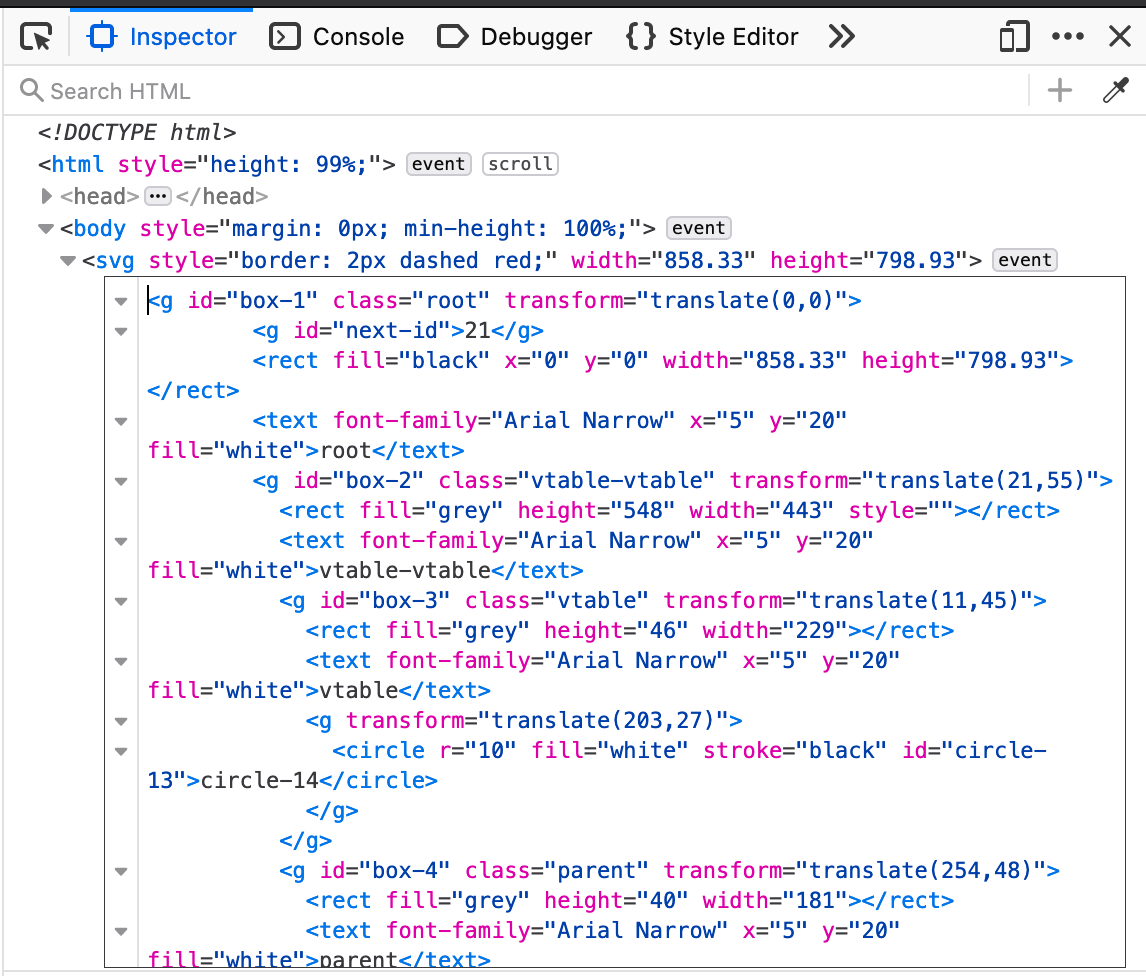
\includegraphics[width=0.8\textwidth]{../html-inspector.png}
  \caption{To save the state of the system, the SVG group corresponding to the \texttt{root} box is copied and pasted inside the HTML file's \texttt{\textless{}svg\textgreater{}} element.\label{fig:html-inspector}}
\end{figure}

This required a slight change towards an architecture where the all the
data required to reconstruct the system's current state is contained in
the inspector HTML, as opposed to hidden JS properties. Where previously
``boxes'' were created first as invisible JS objects responsible for
some SVG, now it was the other way round. When a rect is clicked, the
system must look at some SVG and interpret it ``on demand'' as a box
(although this helper object, once created, can be cached in the SVG
nodes).

Persistence seems to be a weaker cousin of \textbf{externalisability},
defined in \cite{externalise}. As it stands, the system does not quite
qualify as externalisable. When making changes to the HTML in the
element inspector, the system's behaviour \emph{ought} to adjust to
match, but this is not currently guaranteed. Depending on the ability to
listen for changes in node attributes or children, this may remain the
case.

\hypertarget{the-system-as-a-part-of-the-solution}{%
\section{\texorpdfstring{The Id{} system as a part of the
solution}{The  system as a part of the solution}}\label{the-system-as-a-part-of-the-solution}}

The Id{} system was designed with a goal of eliminating the
``artificial'' distinction between implementation language and end-user
language, by means of a mostly self-defining, or ``meta-circular''
object model. This general way of working on a piece of software ``by
means of itself'' is easy to agree with, even if OOP is not to
everyone's taste. It is an open question whether Id{}'s approach could
be applied to other programming styles.

The allure of meta-circularity here is not merely in being ``cool'', but
that it paves the way to end-user empowerment. This is somewhat
misleading because in Id{}, these ``end-users'' are actually
programmers. However, its purpose is to free a programmer's dependence
on some distant and busy\footnote{Not to mention \emph{unelected?}
  ``Take Back Control!'' (jokes aside, in this context it makes a lot of
  sense.)} language designer. It seems plausible that this is a step on
the way to enabling \emph{creation} of a piece of software which
non-programmers do not depend on us for.

I emphasise that this is the \emph{allure} of Id{}. However, there are
some significant practical issues that must be overcome or clarified
first.

\hypertarget{minimal-descriptions}{%
\subsection{Minimal descriptions}\label{minimal-descriptions}}

The Id{} paper was part of the STEPS project of Alan Kay's
VPRI\footnote{Viewpoints Research Institute}. This project argued that
the immense level of ``accidental complexity'' present in software
implementation could be reduced, and Kay himself dreams of an end result
analogous to a ``Maxwell's Equations'' of software. That is: the
behaviour of electromagnetic fields can be represented in four short
equations that fit ``on a T-shirt''.

A self-hosted LISP interpreter fits on a page. Could we aim at a similar
``fundamental description of software'' that fits on something less than
millions of lines of code?

This argument as stated suffers by glossing over an important fact.
Maxwell's equations certainly do fit onto a T-shirt, but most people
will not be able to explain what they mean. What typically amounts to
years of study is compressed into those mathematical symbols, and the
learning material involved most certainly does \emph{not} fit on a
T-shirt. The obvious \emph{reductio ad absurdum} is where we encapsulate
these equations under a single symbol\footnote{In fact, this is almost
  achieved by the formalism of Geometric Calculus, which reduces them to
  only one equation.}, \(\mathcal{M}\). \(\mathcal{M}\) is defined as
``Maxwell's Equations are true''. Ta-da---this fits on a coin, but good
luck doing anything with it.

I say this not to dismiss the argument, but to highlight the
\emph{actually hard part} of getting a ``concise description'' of some
system; defining complexity away into a symbol helps us no more than
naming the solution to an equation ``\(x\)''. There is a connection with
data compression: even if the data is successfully compressed into a
smaller file, the size of the compression \emph{program} should be added
as well. What matters is to reduce the \emph{combined} size of notation
and substrate.

Further, there is perhaps a risk of optimising for \emph{formal} rather
than \emph{practical} minimality (e.g.~the Turing machine). Id{}'s
``minimality'' does not necessarily translate into ``simplicity''. It
suffers from the same \emph{cognitive} complexity, or need for study, as
Maxwell's Equations; I cannot stress enough the amount of effort I have
put in to wrap my head around the self-referential ``vtable vtable'' and
the task of self-implementation. An overall better system might be one
which is easier to pick up or understand, even if the number of formal
objects is not as minimal.

In the conclusion of \cite{OROM}, the authors note that ``it is not
necessarily a friendly model for hand-written code'', suggesting its use
as a compilation target. In a similar vein, it could function as the
kernel of a much more familiar system (on the surface)---it is, after
all, supposed to be a vehicle that other things sit on, rather than the
final user interface itself. In fact, this is precisely the approach set
out in the related paper \cite{COLAs}.

\hypertarget{self-implementation}{%
\subsection{Self-implementation}\label{self-implementation}}

Said related ``COLAs'' paper expands on Id{}, giving it a ``structural''
role complemented by a LISP-like programming language.
Section\textasciitilde{}6.1 sketches out the intended ``bootstrapping''
process, ending with a self-sufficent, self-hosting version of the
system.

However, this task again suffers from the same cognitive complexity as
any other self-referential circle. This is even more so for me, having
made the complexity of graphics and interaction somehow still ``part of
the system''. Figuring out exactly how the authors' bootstrapping
process of their wholly \emph{language-based} system maps on to my task
is, as far as I know, uncharted territory.

Finally, in \cite{crit-semprola}, there is a warning against ``obsession
with completely homogenous systems'' written in themselves. If this
approach is doomed then obviously I want to take a different one, but
the argument against it seems to hinge on what constitutes ``failure''.
It considers Smalltalk and LISP as ``unsuitable'', yet the authors of
Id{} clearly think the opposite. The disagreement probably hinges on
``unsuitable for \emph{what}?'' and it would be clearer if the following
two questions were answered:

\begin{enumerate}
\def\labelenumi{\arabic{enumi}.}
\tightlist
\item
  Is there a difference in (final, intermediate) goals between the two
  views?
\item
  Could systems like Id{} and COLAs plausibly succeed at their own
  stated goals?
\end{enumerate}

\hypertarget{conclusions-and-future-work}{%
\section{Conclusions and future
work}\label{conclusions-and-future-work}}

\hypertarget{what-did-it-take-and-why}{%
\subsection{What did it take, and why?}\label{what-did-it-take-and-why}}

It takes a lot of work to create in a substrate that feels suited to the
domain. Much of this work involves filling in the machinery necessary to
an awful lot of software, rather than the ways one's domain
\emph{differs from} this common case.

In an ideal world, there would be no accidental complexity, no
boilerplate, no polyfilling. But this can't be the same as saying there
would be no \emph{work} to do---that sounds like a world where
\emph{essential} complexity has also been removed.

Instead, we can note that software ecosystems typically centre around a
``core'', such as a language, with a surrounding ``periphery'', such as
libraries not bundled with the core language. The core (language syntax,
semantics, standard libraries) acts as a common platform uniting the
community; the periphery consists of functionality that is not
``built-in'' to this core, both realised as software (e.g.~libraries),
and that which is as-of-yet unrealised or nonexistent.

There is a constant process of negotiation determining what should be
part of the shared core versus the responsibility of the periphery. But
at any given time, every community draws the line somewhere.

To a first approximation, what is ``built-in'' encompasses the features
and concerns that are \emph{common} to the entire community. Features
that are of minority or niche use belong outside; it is one's own
responsibility to implement them, or to integrate with an existing
implementation.

Perhaps in an ideal world, someone could realise their vision in
software by focusing all their effort on what makes their idea
\emph{unique}, or what is \emph{idiosyncratic} to it. In other words,
they would only be responsible for that part of their idea which:

\begin{enumerate}
\def\labelenumi{\arabic{enumi}.}
\tightlist
\item
  It would be unrealistic to expect the wider community to have
  \emph{thought of already}, and
\item
  It would be unfair to expect the wider community to \emph{build on his
  or her behalf.}
\end{enumerate}

If the core Web platform (particularly JavaScript) is meant \emph{for}
supporting ``web apps'', and this is indeed how it is used, then it
seems it has not yet fully absorbed the functionality common to this
usage. At present, this is simply a surprise, or a puzzle, and it might
simply be a matter of time before it catches up.

Nevertheless, I wanted to explicitly highlight the obstacles one is
likely to meet when starting from this platform. They include not only
those specific to the Web, but also issues that occur far more widely
(e.g.~monopoly ontologies.) I showed how, in the short-term, we can
overcome these with solutions intended to be domain-appropriate to their
use (within the syntactic limits of JavaScript).

\hypertarget{what-next}{%
\subsection{What next?}\label{what-next}}

Id{}/SVG more or less realises my desired substrate for implementing
Id{}. However, there is one major area I failed to make
domain-appropriate. Despite representing the ``data'' parts of the
system as I wanted, the \emph{computational} parts of Id{} were just
transplanted into the text boxes as source code. I will reiterate that
this is \emph{sometimes} suitable, but not always, and it would be worth
exploring alternative ways to express some of it in the substrate I
have. Having JavaScript code that the user can modify also seems to mess
up the browser's debugger when stepping through it.

Still, in this mostly-suitable substrate for Id{}, I can continue with
my project of seeing whether the \emph{allure} of \cite{COLAs} can be
saved from the text-based ``hidden world'' limitation that pervades it.
The obvious next step is attempting ``self-implementation''. This is
desirable is because I still have not escaped my text editor. Any
changes to my Id{}/SVG substrate (of nested box drawing) require going
back to the script files; I still cannot take advantage of the system I
have developed, to ease its own development. In the words of
\cite{COLAs}, I wish to make it so that the original JavaScript files
can be ``jettisoned without remorse''.

In Section\textasciitilde{}\ref{retained-mode-vector-graphics}, I
touched on how everyone with a browser has access to a powerful vector
graphics editor (SVG) locked behind a completely inappropriate UI (the
JS Console). It is similar for 3D graphics (WebGL), and sound and music
(Web Audio). Similar observations are made about ``native'' OS apps in
\cite{prog21-dyn}. Unfortunately for that domain, the interface that
unlocks your operating system's range of functionalities---batch-mode
compilation---is quite far from the affordances of the (interactive) JS
Console.

I intend to use Id{}/SVG to ``tame'' SVG and other JavaScript APIs, with
some minimal on-demand visualisation in the large portion of the screen
next to the JS console. This is an attempt to generalise the ``rect
controls'', which allow the obvious geometric properties of a
\texttt{\textless{}rect\textgreater{}} to be directly manipulated
(Section\textasciitilde{}\ref{context-appropriate-ontologies}). Giving
Id{} access to Web technologies in this way is essential for evolving it
into a \emph{fully-featured} self-changeable software environment, which
could allow as much domain-specifc representation as its user wishes.
